The objective of this project is to implement a Jenga-playing robot system involving a human opponent. Our solution will utilize 3D computer vision to develop scans of the tower's state, and a vacuum gripper to grip blocks. The human opponent will take turns with the robot performing block pulls and placing them at the top of the stack. The goal isn't necessarily to defeat the human opponent, but build a system capable of make multiple moves prior to the tower collapsing. 

\subsection{Purpose and Use}
This project serves as an interactive demonstration of computer science concepts with the goal of inspiring the next generation of scientists \& engineers. This product is designed to engage K-12 students at showcases and university outreach events. Students are expected to engage with the product by taking turns with the robot in a fun, friendly game of Jenga.

\subsection{Intended Audience}
This product is intended to be used by the university, College of Engineering, or the Computer Science \& Engineering Department as a recruiting tool for future engineering students. Making this product available commercially to other universities and companies is possible. Though, as this is an end-to-end system designed to demonstrate the possibilities as a STEM student at UT Arlington, it is intended to be administered on behalf of the university. The end-user of this system is a member of the general public. Mattel$\circledR$ states that Jenga is appropriate for players ages six and up.

\begin{figure}[h!]
	\centering
   	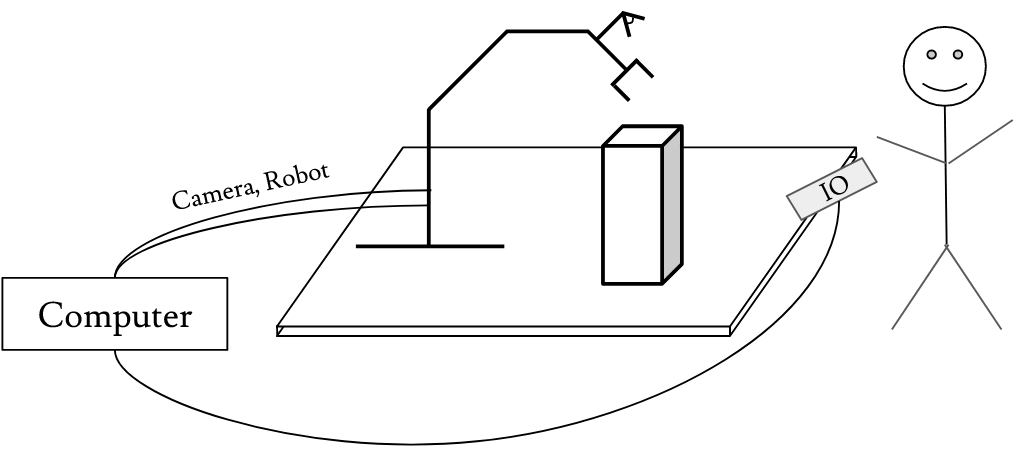
\includegraphics[width=0.90\textwidth]{images/system_setup}
    \caption{System concept drawing}
\end{figure}
